\chapter{Introduction}
\section{Neural Networks}

Deep Neural networks are a very popular machine learning model these days. They are known to be very expressive, leading to low bias. They are especially useful for learning from very large data sets. A deep neural net is shown in figure \ref{neural}. It is made by connecting layers of 'neurons'. Each neuron is a nonlinear function transforming the weighted sum of its inputs:
\begin{equation*}
      y = \sigma(w_1x_1+w_2x_2+...+w_nx_n)
\end{equation*}
This is the McCulloch-Pitts neuron model. The most commonly used activation function $\sigma$ is the Rectified Linear Unit (ReLU):
\begin{equation*}
      \sigma(x) = x^+ = \max(0,x)
\end{equation*}

   \begin{figure}[b]
	\centering
	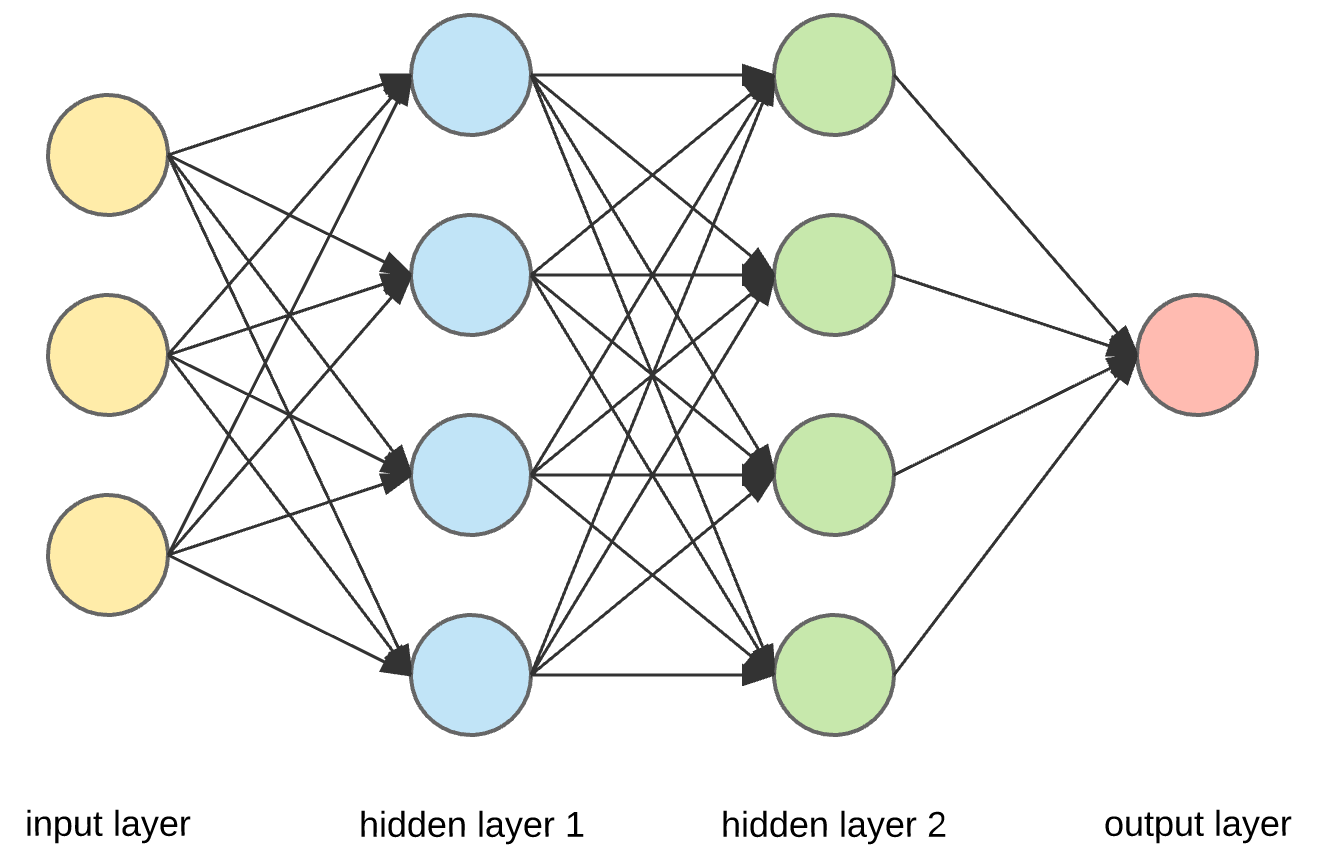
\includegraphics[width=0.49\textwidth]{network}
	%\caption{Feedforward Deep Neural Network. (Retrieved from https://towardsdatascience.com)}
	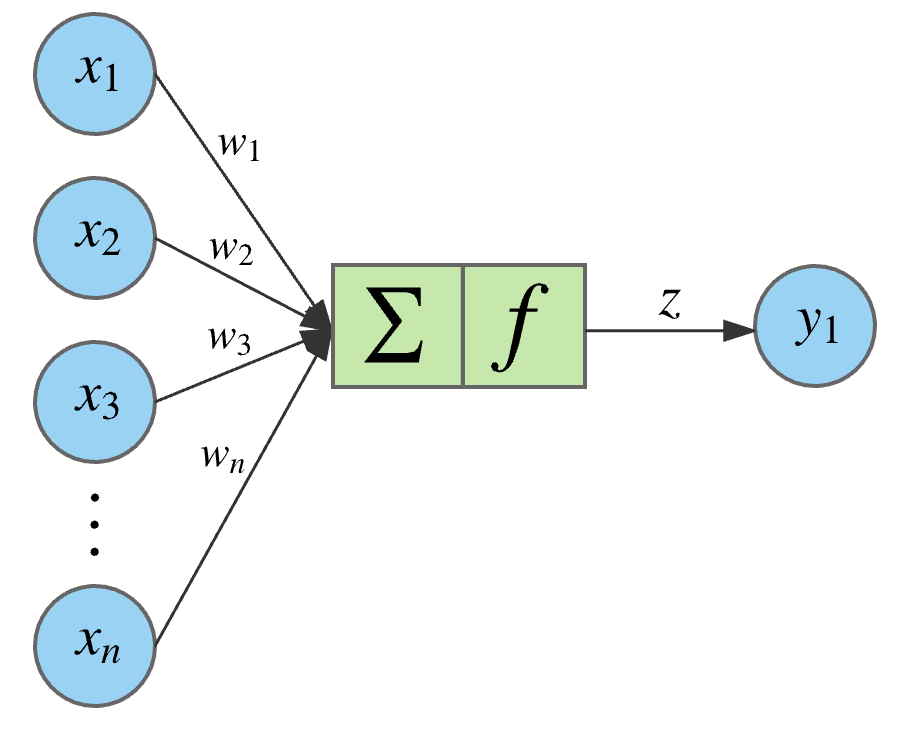
\includegraphics[width=0.49\textwidth]{neuron}
	\caption{Feedforward Deep Neural Network and Single Neuron - McCulloch-Pitts model. (Retrieved from https://towardsdatascience.com)}
	\label{neural}
	\end{figure}

\newpage
\section{Neural Networks as Dynamical Systems}
A neural network can also be expressed as a function in matrix notation: 
\begin{equation*}
         f(W,x) = W_H\sigma(W_{H-1}\sigma(...W_1\sigma(W_0x)...))
\end{equation*}
where $W_n$ are the matrixes of the connection weights.

Training of this network is then done by minimizing the loss function:

\begin{equation*}
\begin{aligned}
& \underset{W}{\text{minimize}}
& L(W) &= \sum\limits_{j=0}^{N}||f(W,x^j) - y^j||^2 \\
\end{aligned}
\end{equation*}

The usual algorithm is called backpropagation. This algorithm has two steps: first the output of the network is calculated using the current weights. Then the error is propagated backward and the gradient is calculated. Then any gradient descent method can be used to find the step update.

A neural network can also be interpreted as a dynamical system where every layer is a state.
\begin{equation*}
	\begin{aligned}
	x_0 &= x \\
	x_{k+1} &= \sigma(W_kx_k), & k = 0,...,H-1 \\
	y &= W_Hx_H \\
	\end{aligned}
\end{equation*}
In this way optimization methods from Control Theory can be applied. In particular, training a neural network with ReLU activation function is equivalent to solving the following Optimal Control Problem (OCP)
\begin{equation*}
	\begin{aligned}
	& \underset{W}{\text{minimize}}
	& & \sum\limits_{j=0}^{N}||W_Hx_H^j - y^j||^2 \\
	& \text{subject to}
	& & x_{k+1}^j = \max(W_kx_k^j,0), &k = 0,\ldots,H-1,j = 1,\ldots,N
	\end{aligned}
\end{equation*}

There are two approaches to solving an OCP. First is the sequential approach, where the states are eliminated using the dynamics. This is equivalent to the backpropagation algorithm which is the current standard method.

The other approach is the simultaneous approach, where the states are kept as variables and the dynamics are kept as constraints. In control theory this approach often works better for highly nonlinear problems, which is certainly the case for training neural networks. The simultaneous approach is novel to neural networks and will be the topic of this thesis.

The disadvantage of this method is the number of variables that need to be optimized is much larger. For a fully connected neural network of width $W$, each layer will contain $W^2$ weights. Combined with a depth $D$, that gives approximately $W^2D$ weight variables to be optimized for both the backpropagation and simultaneous approach. Adding the states as variables however adds another $WDN$ variables, where $N$ is the number of samples in a training batch. The advantage of this method is that relaxing the states makes the problem more smooth, and will hopefully allow the optimization to converge more often to a good solution and not land in a bad local minimum.
